\section{Experiment Pipeline}
\label{sec:methods/section_c}

Once we selected the parameters for YOLOv3 and SORT, we are ready to run the experiment for taking measurements. The experiment will involve two cases of taking measurements; running the object detector and tracker on the uncompressed video sequences and compressed sequences. For the case of compressed sequences, we apply HEVC video compression of version HM16.20 at different quantization parameter (QP) and motion search range (MSR). Table \ref{qp_msr_range} shows the range of QP and MSR attempted for the experiment.
\begin{table}[]
    \centering
    \begin{tabular}{|c|c|}
        \hline
        HEVC parameter & Range of values \\
        \hline
        \hline
        QP & [18, 22, 26, 30, 34, 38, 42, 46] \\
        \hline
        MSR & [8, 16, 32, 64] \\
        \hline
    \end{tabular}
    \caption{Caption}
    \label{tab:qp_msr_range}
\end{table}
For the case of uncompressed sequences, we don't apply HEVC compression but run object detector and tracker directly on the sequences. The uncompressed sequences from Table \ref{tab:seq_list} were used but we excluded the training sequence of Class C PartyScene since we have used this sequence to tune the parameters to optimize the detector and tracker. Therefore, there are totally 12 sequences that were used for the analysis. Figure \ref{fig:experiment_pipeline} shows the pipeline for the experiment and each step is explained in the following steps.

% \begin{myfont}
% \centering
% QP = [18, 22, 26, 30, 34, 38, 42, 46], MSR = [8, 16, 32, 64]
% \end{myfont}


\begin{enumerate}
    \item \textbf{HEVC Encoding}: The experiment starts with applying HEVC encoding to the uncompressed sequences and generating the compressed bitstreams. Low Delay Encoding is used for encoding. Encoding is the process that took the most amount of time in the entire pipeline, so we encoded all the possible combination of QP and MSR and saved all the compressed bitstreams before applying decoding.
    \item \textbf{HEVC Decoding}: After obtaining all the compressed bitstreams, we apply HEVC decoding to the bitstreams and output the decoded sequences in YUV420 format.
    \item \textbf{YUV420 to RGB24 color conversion}: Since the YOLOv3 object detector accepts in RGB24 format, we convert the decoded sequences in YUV420 to RGB24 format in .png files.
    \item \textbf{Running YOLOv3 and SORT}: Once obtaining the decoded sequence in RGB24, we run the object detector and tracker to obtain the tracking results in MOT benchmark format. 
    \item \textbf{MOT metrics evaluation}: To assess the tracking performance, we input both of the tracking results and ground truth, and the software \cite{heindl_cheindpy-motmetrics_2021} will generate the tracking performance result.
\end{enumerate}
We ran YOLOv3 and SORT to detect and track each class ID as shown in Table \ref{tab:seq_list} as single class tracking and also detect and track all available object classes as multiple classes tracking. In other words, we performed a single class multiple object tracking and multiple classes multiple objects tracking.
\begin{figure}[!htb]
  \centering
  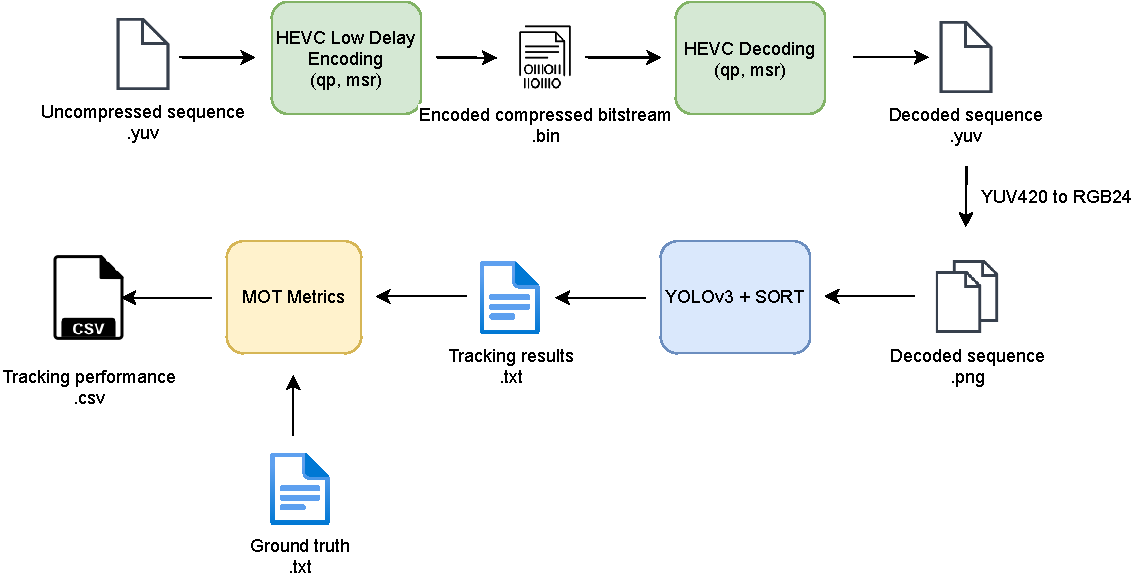
\includegraphics[width=1.0\linewidth]{img/experiment_pipeline.pdf}
  \caption[Pipeline for the experiment]
  {Pipeline for the experiment.}
  \label{fig:experiment_pipeline}
\end{figure}

